\documentclass{bioinfo}
\copyrightyear{2014}
\pubyear{2014}

\begin{document}
\firstpage{1}

\title[HPO Annotator]{Automated HPO-Annotations for newly sequenced proteins by homology inference}
\author{K. Nagaraj$^{1}$, M. Hanumanthappa$^{1}$, O. Tarabai$^{1}$, S. Seitz$^{1}$}
\address{$^{1}$Fakul\"at f\"ur Informatik, Boltzmannstr. 3, 85748 Garching}


\history{Received on 28.02.2014}
\editor{Associate Editor: I12 - Department for Bioinformatics and Computational Biology - Fakult\"at f\"ur Informatik, Boltzmannstr. 3, 85748 Garching}

\maketitle

\begin{abstract}

\section{Motivation:}
Rapid genome sequencing and high-throughput technology, automatic function prediction for a novel sequence is an essential matter in bioinformatics. Automatic annotations based on local alignments suffer from several drawbacks \citep{Ori06}. With our de novo method we try to improve the precision and recall of automatic annotations.
\section{Results:}
Text  Text Text Text Text Text Text Text Text Text  Text Text Text Text Text Text Text Text Text  Text Text Text Text Text Text Text Text Text  Text Text Text Text Text Text

\section{Availability:}
The webinterface for our created prediction-method is available at https://dataminer.informatik.tu-muenchen.de/~omar.tarabai/.

\section{Contact:} \href{name@bio.com}{name@bio.com}
\end{abstract}

\section{Introduction}
In the databases many proteins are found for which the sequence is known, but the function is still not determined. With the increasing number of sequences, caused for example by genomic scale projects, traditional experimental approaches have become outpaced. This leads to the need for rapid and reliable functional annotation methods \citep{Rodrigues07}. 

Many different approaches have been taken annotate protein function by computational methods, including methods based on sequence, expression, interaction and tertiary structure. Despite this taken effort and the following increase of number and variety of prediction methods, automated annotation remains difficult. Reasons for these difficulties can for example be found in the inherent limitations of current tools and databases or the ambiguity of the definition of function itself \citep{Rodrigues07}.

To overcome this problems and to be able to annotate protein function without relying on tertiary data, this method is created to reliably predict protein function by sequence alone.

%TODO what to do with this 2 paragraphs?
%Genomic scale projects have compounded the need for rapid and reliable functional annotation methods. Traditional experimental approaches have become outpaced resulting in an ever-increasing proportion of missing annotations. Computational approaches, including those based on sequence, expression, interaction and tertiary structure, have the potential to impact the growing annotation deficit.
%
%Despite a recent increase in the number and variety of prediction methods, the computational annotation of protein function remains difficult. This stems from a combination of issues such as the inherent limitations of current tools and databases, the difficulty of assessing the predictive power of different methods and more fundamental problems related to the ambiguity of the definition of function itself. %TODO http://www.biomedcentral.com/1471-2105/8/S4/S1 - real paper!

\section{Material \& Methods}

Our method mainly relies on using protein sequence similarity as an indicative of functional similarity in order to transfer Human Phenotype Ontology (HPO) annotations from known to unknown protein sequences. Therefore, in order to achieve a reasonable prediction, we needed a set of properly annotated and reviewed protein sequences to use as a reference database. For this we used...

We used BLAST 2.2.26 \cite{blastweb} which is a widely-used tool for protein sequence alignment, it takes as input a pre-generated database of reference protein sequences and a target sequence. It employs a heuristic algorithm to search the reference database for sequences that are most similar to the target sequence. Its main output is the top N hits sorted from the most similar to the least similar protein sequence. Additionally, it outputs a number of other values defining statistics about the degree of similarity discovered, most relevant to our method is the "bit score" value which is a statistical measure of how good the calculated sequence alignment is \cite{blastscore}.

Our core algorithm takes three parameters as input, \textit{sequence} which is the target protein sequence string, \textit{hits N} which is the number of hits (positive integer) returned by blast to be used in the prediction, \textit{threshold T} which is cut-off value (real number between 0 and 1 inclusive) for the predicted annotation terms according to their confidence parameter.

The algorithm starts by querying BLAST for the top \textit{N} hits for the target sequence against our pre-generated sequence database. For each of the resulting hits, we construct the full HPO tree from the set of HPO annotation terms corresponding to the hit protein, each term in the tree is labelled with the BLAST "bit score". The resulting N trees are merged together into a single prediction tree, the merging is a simple union operation, scores of the same term found in more than one tree are added together in the final prediction tree. Scores are then normalized to the [0,1] range using equation~(\ref{eq:01}) where $S$ is the predicted term score, $S_{min}$ and $S_{max}$ corresponding to the minimum and maximum scores found in the predicted tree respectively. As the final step, the threshold \textit{T} is applied to the predicted tree by removing any terms with a score lower than the threshold. The output of the algorithm is the list of "leaf" terms in the final tree and the corresponding normalized score as the term \textit{confidence} value.

\begin{equation}
S_N = \frac{S - S_{min}}{S_{max} - S_{min}}
\label{eq:01}
\end{equation}

TODO: add "default tree" idea.

\section{Results}

An experiment was performed to arrive at the optimum values for the free parameters \textit{N} and \textit{T} described in the previous section. We ran the algorithm using as input each of the protein sequences that we have HPO annotations for and different values of \textit{N} (5 to 8 inclusive) and \textit{T} (0 to 1 inclusive with a step of 0.1). Since the target sequences used are present in the reference database, we altered the algorithm to query blast for the top $N + 1$ hits instead and removed the target protein from the result set. After each run, we compare the resulting prediction tree against the actual prediction tree and calculate the \textit{precision}, \textit{recall} and \textit{F-value} using equations \ref{eq:02}, \ref{eq:03} and \ref{eq:04} respectively, these values are then averaged over the whole set of target sequences used. Figure \ref{optim} shows the resulting \textit{F-value} for the different values of \textit{N} and \textit{T}. Since \textit{F-value} is considered a compromise between \textit{precision} and \textit{recall}, we use it as an indicative of performance, best result was achieved at \textit{N} = 7 and \textit{T} = 0.2 with an \textit{F-value} = 0.2842.

\begin{equation}
precision = \frac{true positive}{true positive + false positive}
\label{eq:02}
\end{equation}

\begin{equation}
recall = \frac{true positive}{true positive + true negative}
\label{eq:03}
\end{equation}

\begin{equation}
F-value = \frac{2 \times precision \times recall}{precision + recall}
\label{eq:04}
\end{equation}

\begin{figure}[!tpb]
\centerline{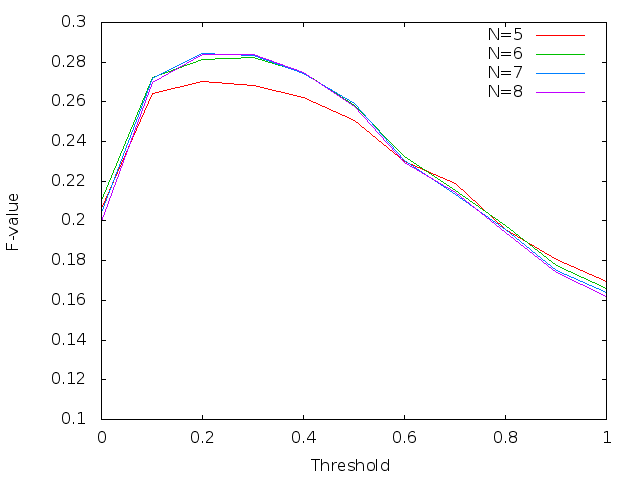
\includegraphics[scale=0.4]{bilder/optim.png}}
\caption{Optimization experiment results}
\label{optim}
\end{figure}

\section{Discussion}


\section*{Acknowledgement}
Without the great help and guidance by the Rostlab, and every group member there, we wouldn't have been able to succeed in creating our method. Also we'd like to thank the Rostlab for letting us access their computers and equipment.

\begin{thebibliography}{}

\bibitem[BLAST]{blastweb} BLAST: Basic Local Alignment Search Tool. \href{http://blast.ncbi.nlm.nih.gov/Blast.cgi}{http://blast.ncbi.nlm.nih.gov/Blast.cgi}

\bibitem[BLAST score]{blastscore} BLAST Scores and Statistics. \href{http://www.ncbi.nlm.nih.gov/books/NBK21097/\#\_A614\_}{http://www.ncbi.nlm.nih.gov/books/NBK21097/\#\_A614\_}

\bibitem[Rodrigues {\it et~al}., 2007]{Rodrigues07} Rodrigues, Ana PC and Grand, Barry J and Godzik, Adam and Friedberg, Iddo (2007) The 2006 Automated Function Prediction Meeting, {\it BMC Bioinformatics}, {\bf 8}, S1. %source: http://www.biomedcentral.com/1471-2105/8/S4/S1

\bibitem[Ori {\it et~al}., 2006]{Ori06} Sasson, Ori and Kaplan, Noam and Linial, Michal (2006) Functional annotation prediction: All for one and one for all, {\it Protein Science}, {\bf 15}, 1557-1562.

% these following items were predefined in the template:
%\bibitem[Bofelli {\it et~al}., 2000]{Boffelli03} Bofelli,F., Name2, Name3 (2003) Article title, {\it Journal Name}, {\bf 199}, 133-154.
%
%\bibitem[Bag {\it et~al}., 2001]{Bag01} Bag,M., Name2, Name3 (2001) Article title, {\it Journal Name}, {\bf 99}, 33-54.
%
%\bibitem[Yoo \textit{et~al}., 2003]{Yoo03}
%Yoo,M.S. \textit{et~al}. (2003) Oxidative stress regulated genes
%in nigral dopaminergic neurnol cell: correlation with the known
%pathology in Parkinson's disease. \textit{Brain Res. Mol. Brain
%Res.}, \textbf{110}(Suppl. 1), 76--84.
%
%\bibitem[Lehmann, 1986]{Leh86}
%Lehmann,E.L. (1986) Chapter title. \textit{Book Title}. Vol.~1, 2nd edn. Springer-Verlag, New York.
%
%\bibitem[Crenshaw and Jones, 2003]{Cre03}
%Crenshaw, B.,III, and Jones, W.B.,Jr (2003) The future of clinical
%cancer management: one tumor, one chip. \textit{Bioinformatics},
%doi:10.1093/bioinformatics/btn000.
%
%\bibitem[Auhtor \textit{et~al}. (2000)]{Aut00}
%Auhtor,A.B. \textit{et~al}. (2000) Chapter title. In Smith, A.C.
%(ed.), \textit{Book Title}, 2nd edn. Publisher, Location, Vol. 1, pp.
%???--???.
%
%\bibitem[Bardet, 1920]{Bar20}
%Bardet, G. (1920) Sur un syndrome d'obesite infantile avec
%polydactylie et retinite pigmentaire (contribution a l'etude des
%formes cliniques de l'obesite hypophysaire). PhD Thesis, name of
%institution, Paris, France.

\end{thebibliography}
\end{document}
